\documentclass[]{article}
\usepackage{graphicx}
\usepackage{hyperref}
\title{\href{https://www.github.com/}{A New Design of Toy-Gun}}
\author{\href{mailto:jishanshaikh9893@gmail.com}{Jishan Shaikh}}
\date{January 2018}

\begin{document}

\maketitle

\begin{abstract}
A new model of machine gun is presented briefly of which a series of guns can be replaced by a single gun which is light, portable, and atmore powerful than corresponding guns such as AK 47, TA 51, and machine guns too. The Cost of manufacturing of one gun is almost 100\$ which makes it gun with maximum cheap price. No other gun is available till now with such a minimum price and absolute powerful as well.
\end{abstract}

\section{Figures}Five figures are presented here -
\begin{figure}[h]
	\centering
	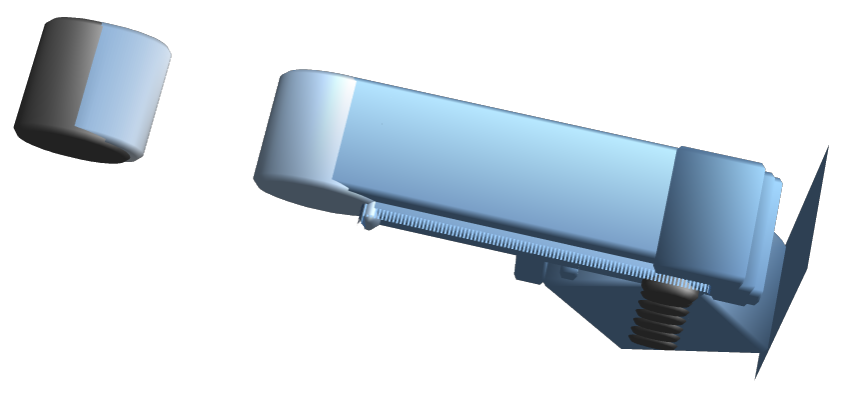
\includegraphics[width=0.5\textwidth]{1.png}
	\caption{Top View}
	\label{image-1}
\end{figure}Five figures are presented here -
\begin{figure}[h]
	\centering
	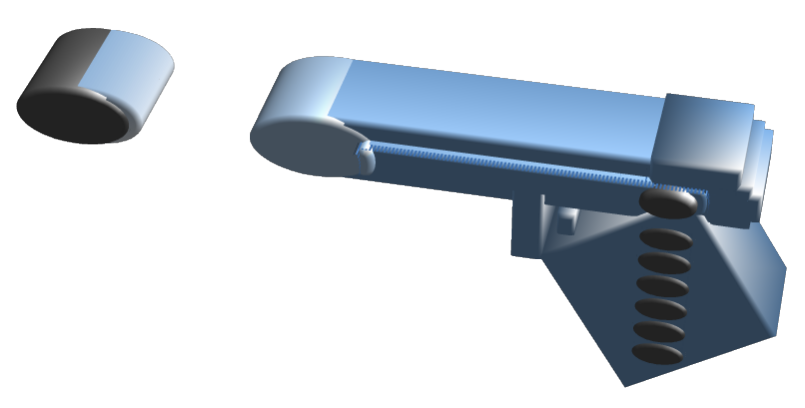
\includegraphics[width=0.5\textwidth]{2.png}
	\caption{Oblique-top View}
	\label{image-2}
\end{figure}Five figures are presented here -
\begin{figure}[h]
	\centering
	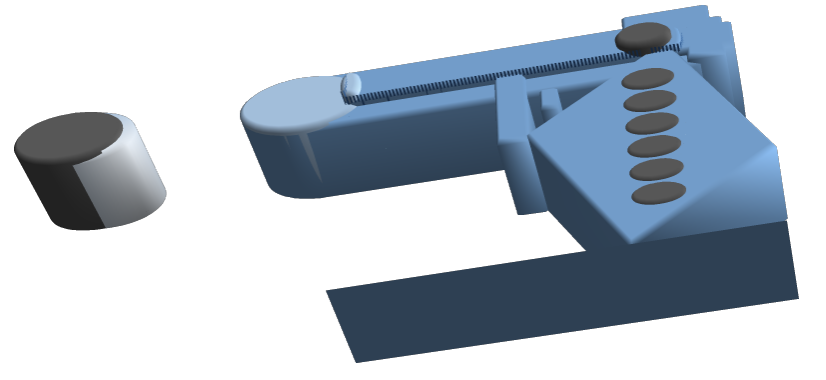
\includegraphics[width=0.5\textwidth]{3.png}
	\caption{Oblique-bottom View}
	\label{image-3}
\end{figure}Five figures are presented here -
\begin{figure}[h]
	\centering
	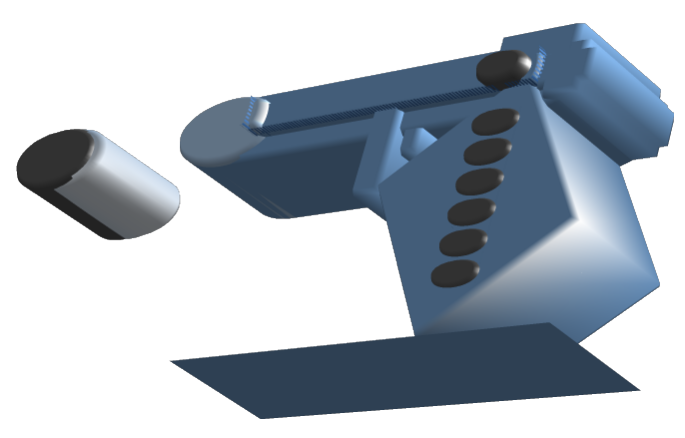
\includegraphics[width=0.5\textwidth]{4.png}
	\caption{Oblique-side View}
	\label{image-4}
\end{figure}Five figures are presented here -
\begin{figure}[h]
	\centering
	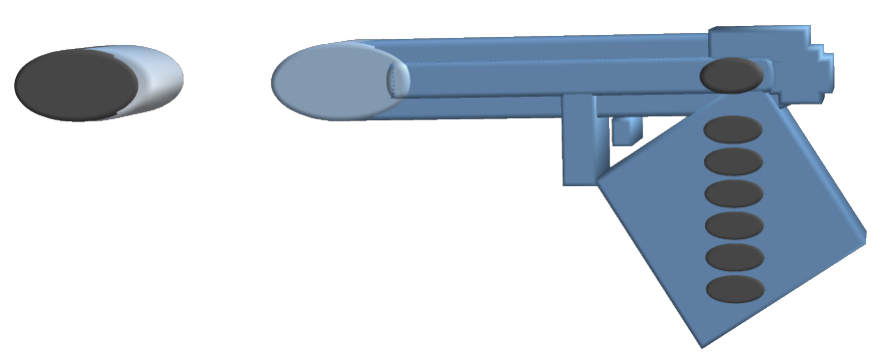
\includegraphics[width=0.5\textwidth]{5.png}
	\caption{Side View}
	\label{image-5}
\end{figure}Five figures are presented here -
\section{Appliactions and Uses}
The proposed gun is capable of shooting upto a range of 100-200 Kms, which is greater than AK 47, AK 51, TA 55, and almost equal to machine gun 100. It can also be replaced by old machine gun established at top of tank numbers 5, 7, and 11. Since, the number of rounds it takes in one time depends on how much we have in single cope, it can also be used in direct one-on-one fighting in extreme areas such as in War, Terrorist-attacks, and in Upbringings of extremists. It has plenty of other applications in Security, Privacy and Licensed-Policing. Its uses makes it a non-beatable gun.
\begin{thebibliography}{10}
	\bibitem{Jis1} Jishan Shaikh. \textit{Design and Analysis of Toys Volume 1-10} Published on Internet at \href{https://www.github.com/JShaikh/}{Github.com}. 11th edition, 2017. ISBN-13 843-543-58-05-13.
\end{thebibliography}

\end{document}
